\documentclass[10pt]{beamer}
\usepackage[UTF8]{ctex}

\usetheme[
%sidebar, % 会在每页左侧加上导航栏,参考 The AAU Sidebar Beamer Theme 设置
% xdblue, % 不选会默认西电红色调,选上会将主题设置为西电蓝色调
% english % 选上,会将图表等标题还原回英文标题
%hidetitle,
%hideauthor,
%hideinstitute,
 ]{XJTUstyle}

\makeatletter
\let\@@magyar@captionfix\relax
\makeatother

\graphicspath{{figures/}}

\usepackage{array}
\usepackage{booktabs}

\AtBeginDocument{%
    \title{面向多CPU集群的\\深度行人重识别研究}
    %\subtitle{子标题}
    \author[李源勋]{%
        \begin{tabular}{ll}
            学\qquad{}生:& 李源勋 \tabularnewline
            指导老师:& 何~~~~晖
        \end{tabular}
    }
    \institute[]{西安交通大学\\计算机~44~班} % 中括号部分为导航栏底所用尽可能精简
    \date{\today}% 时间可自行设置
}
\begin{document}%

%首页标题页
\frame[plain,noframenumbering]{\titlepage}

%目录
\section*{目录}
  \frame {
    \frametitle{\secname}
    \tableofcontents[hidesubsections,sections={<1-6>}]
  }

\pagenumbering{arabic}
\section{项目背景及内容}
随着视频监控技术的发展,无人值守的视频监控设备被越来越普遍地部署在国民社会的各个方面,在
公安、交通、智能楼宇、金融、司法、教文卫等领域都有着不可替代的作用。具体的应用场景包括平
安城市、卡口系统、工地监控、自助银行、监狱劳教和学前教育等。

在视频监控领域一个很重要且极具挑战性的问题是行人的重识别。行人重识别,指的是在多个视野不
重叠的监控视频中,重新识别那些之前出现过的行人,即把当前行人与之前已标记的人物相对应。该
工作的实现可以为人物搜索、特定人物跟踪等应用提供强有力的支持,进而应用在平安城市、工地监
控、学前教育等场景。

行人重识别技术在实际应用中受诸多因素的影响,包括摄像头的部署位置、成像质量以及摄像头数量
等等。面对一个从未部署过摄像头的监控场景,一个优秀的摄像头位置部署方案可以实现监控范围无
死角、行人重识别准确率高以及跨摄像头持续跟踪的连续性强。摄像头的成像质量受其自身的性能参
数影响,同时也受部署位置的光线条件影响。在理想情况下,摄像头的数量越多,得到的行人信息就
越多,更有利于行人重识别算法的实施。但是在预算有限的情况下,摄像头的数量不可能无限增加。
因此,如何选择摄像头的数量及其部署位置,使得行人重识别算法的性能最大化,便成为一个极具现
实意义的研究问题。

要实现行人的重识别需要借助计算机视觉领域的技术。目前的计算机视觉算法的前沿关注点主要集中
在深度学习技术。由于深度学习的海量计算需求和GPU强大的并行计算能力,大部分深度学习模型都
是借助GPU来调整模型参数。然而使用GPU进行运算也存在许多问题,例如GPU设备通常比较昂贵,
且少见于嵌入式设备中。同时GPU的显存普遍不高,限制了模型的规模以及每一批次数据的规模。与
此同时,多CPU集群具有硬件成本低、搭建方式灵活以及部署广泛等优点,然而对于深度学习算法在
多CPU集群上的研究与应用少之又少。因此,有必要对深度学习算法在多CPU集群上的性能表现进行
深入的调查、分析和研究。

基于上述研究背景及动机,本项目的主要研究内容和贡献如下:

\begin{enumerate}
\item 深入理解论文\cite{sun2017beyond}的目的、想法和实现方式,并使用PyTorch深度学习框架
复现,达到与原论文接近的实验结果。
\item 研究在预算有限的情况下,摄像头的数量与部署位置对行人重识别算法的影响,并采用强化学习
算法进行摄像头部署位置的选择。
\item 调查、分析和研究深度行人重识别算法在多CPU集群上的性能表现,提出针对多CPU集群环境
的深度神经网络模型的改进策略。
\end{enumerate}

本项目当前的进展:

\begin{enumerate}
\item 搭建了PyTorch分布式环境,完成了论文复现工作,在Market1501\cite{zheng2015scalable}
数据库上进行实验。
\item 实现了 Q-Learning 强化学习算法,选择最优的摄像头部署方案。
\item 将深度行人重识别模型的训练算法改造成适用于多CPU集群的形式。
\end{enumerate}


























\section{项目内容}

\subsection{数据预处理}

    \begin{frame}{数据预处理}
    \begin{block}{}
    \begin{enumerate}
        \item 视频转码
        \item 时间点校正和估计
        \item 视频切割
        \item 行人检测
        \item 人工标注
    \end{enumerate}
    \end{block}
    \begin{figure}
    \centering
    
\includegraphics[width=\textwidth]{figures/label}
    \caption{数据预处理的最终结果}
    \label{fig:label}
    \end{figure}
    \end{frame}

    \begin{frame}{行人检测效果}
    \begin{block}{}
    检测视频画面帧中的行人,输出bounding box。
    使用Facebook开源的Detectron工具,其实现了Mask RCNN框架。
    \end{block}
    \begin{figure}
    \centering
    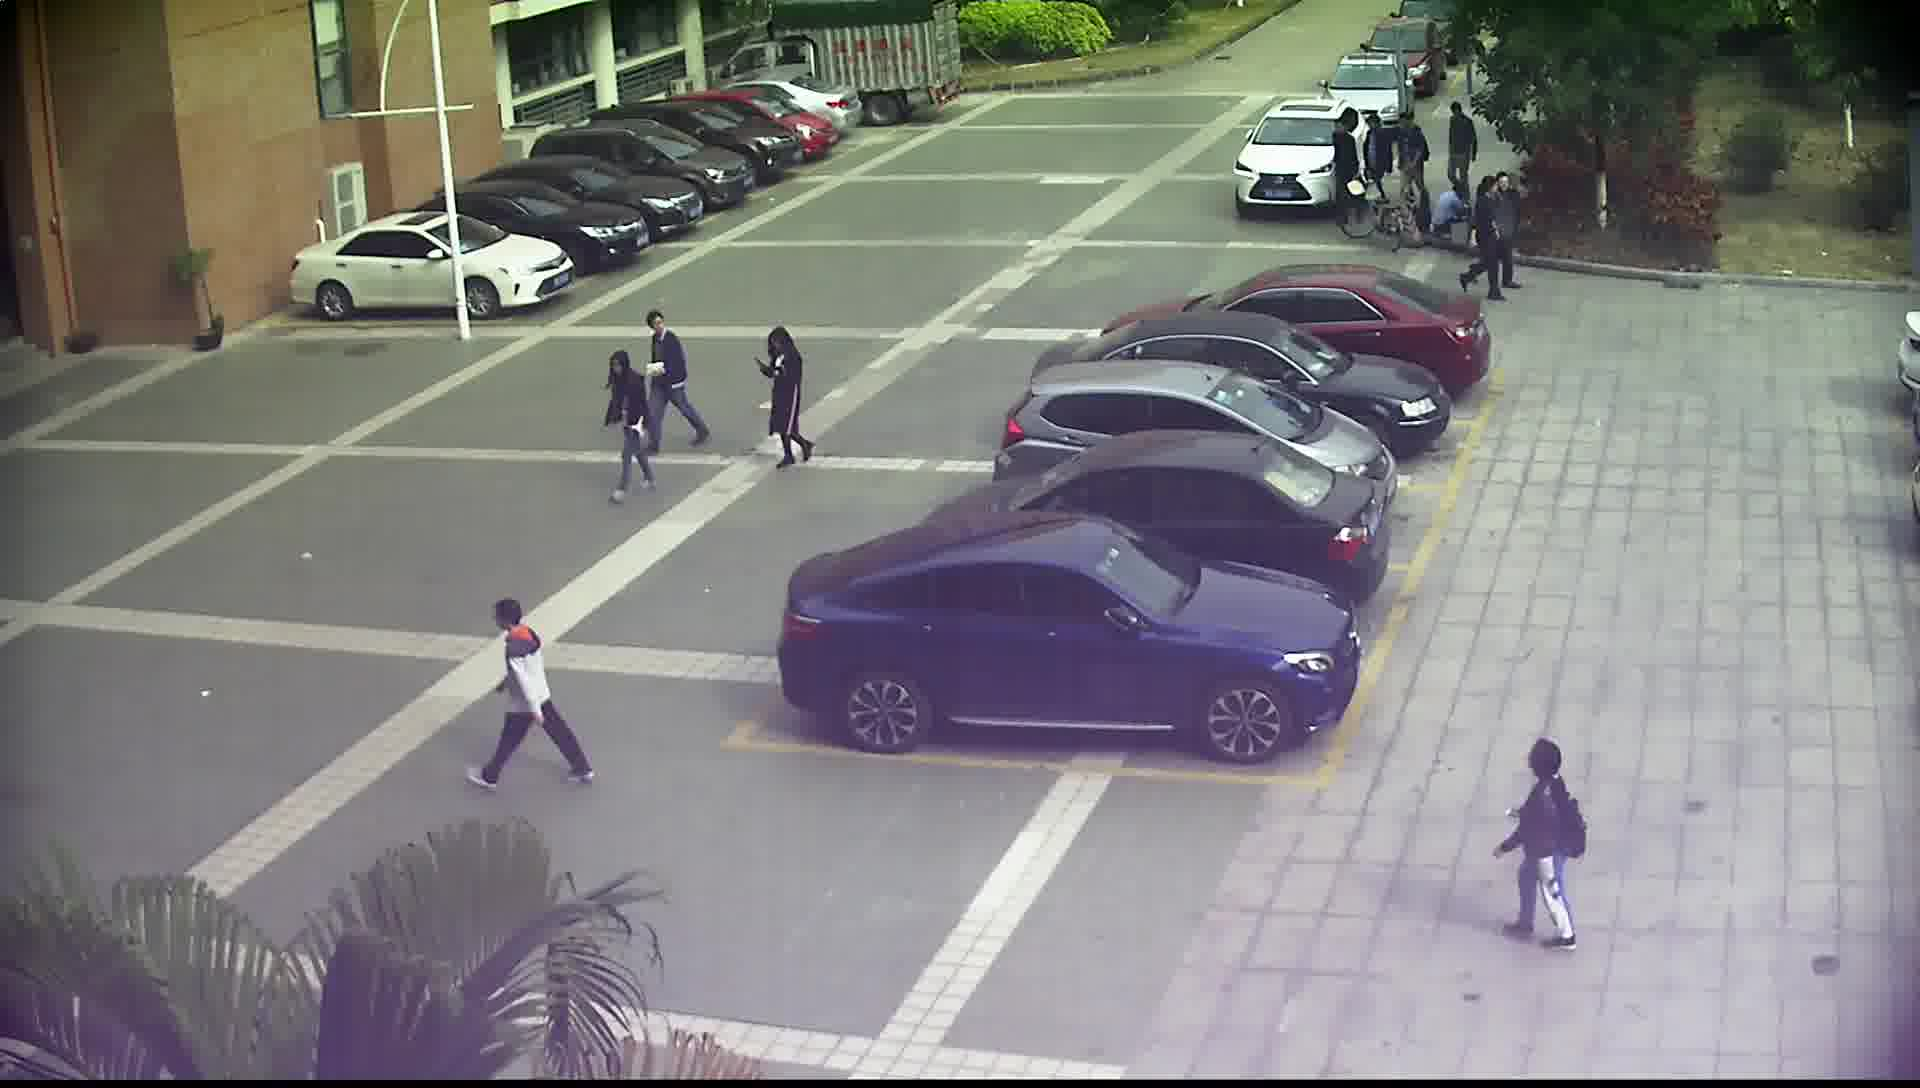
\includegraphics[width=0.3\linewidth]{figures/1-2_5_151.jpg}~
    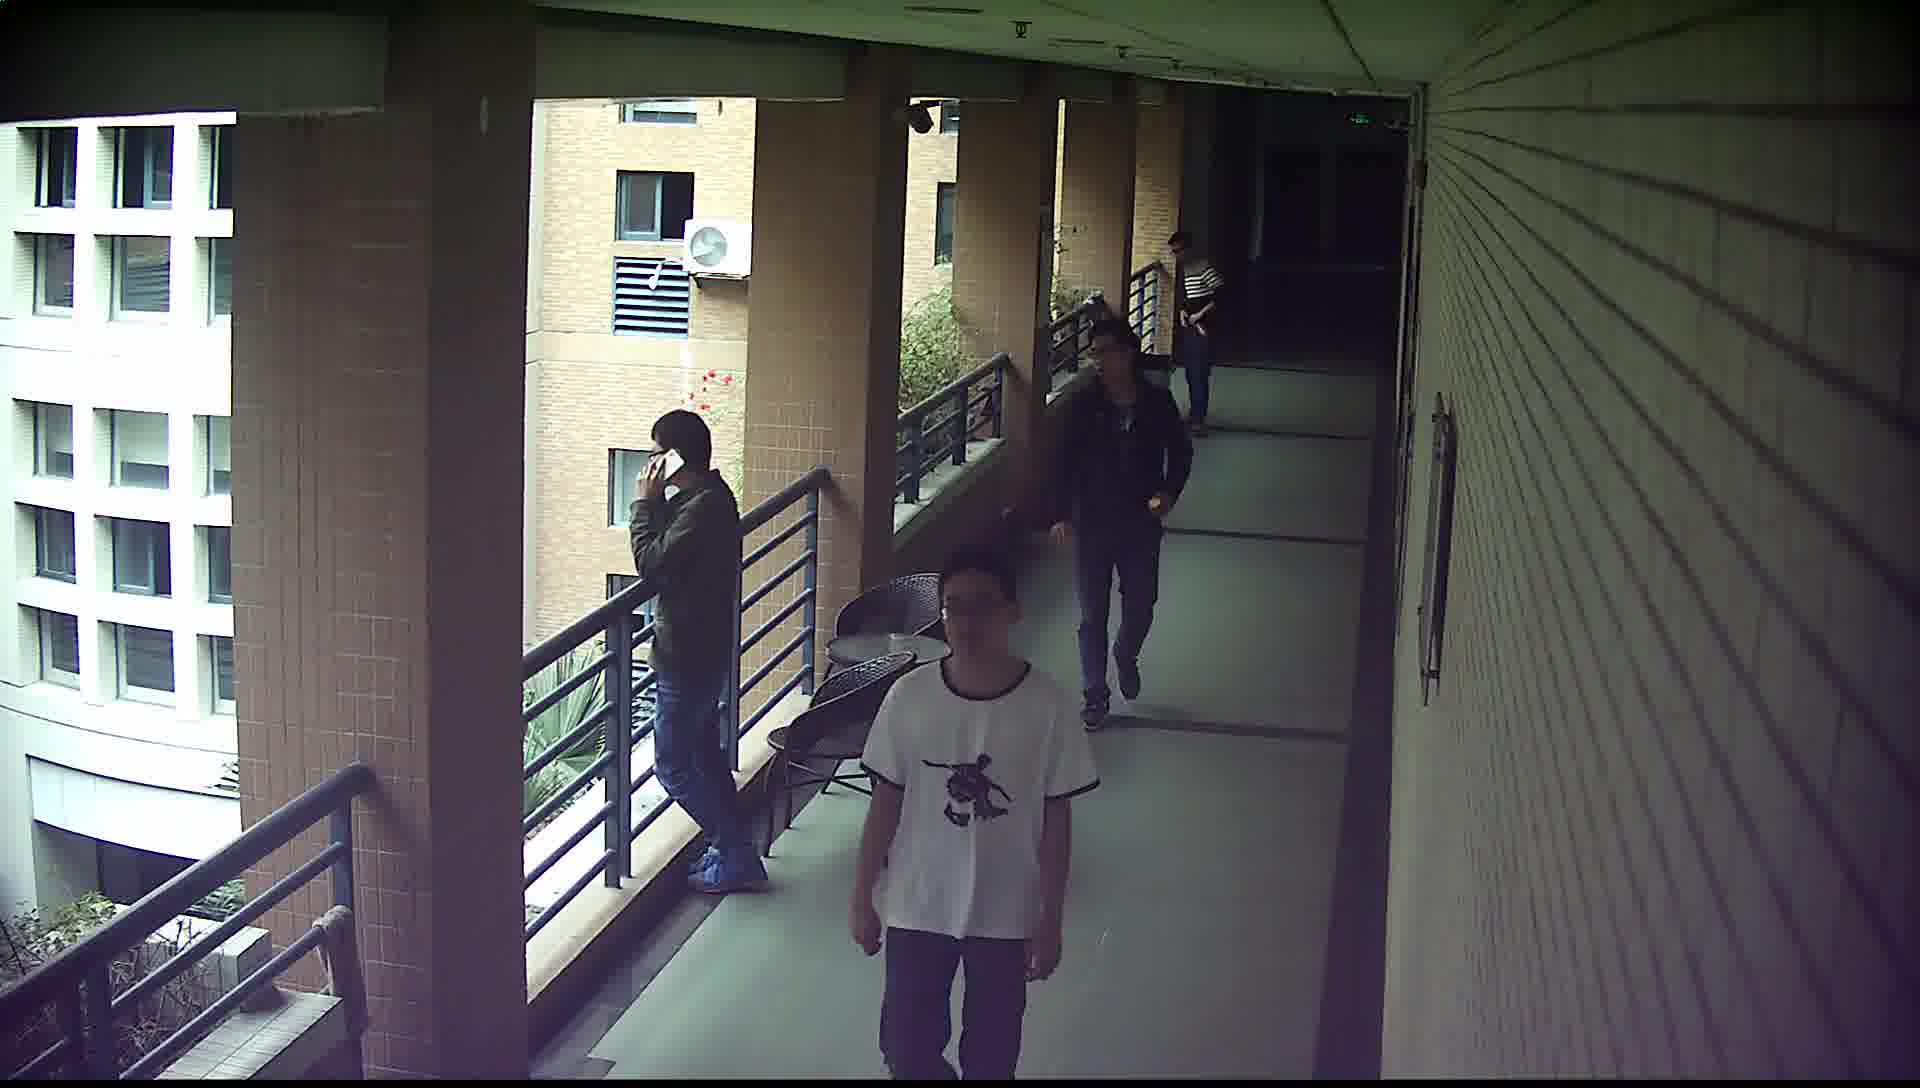
\includegraphics[width=0.3\linewidth]{figures/3-7_10_394.jpg}\\
    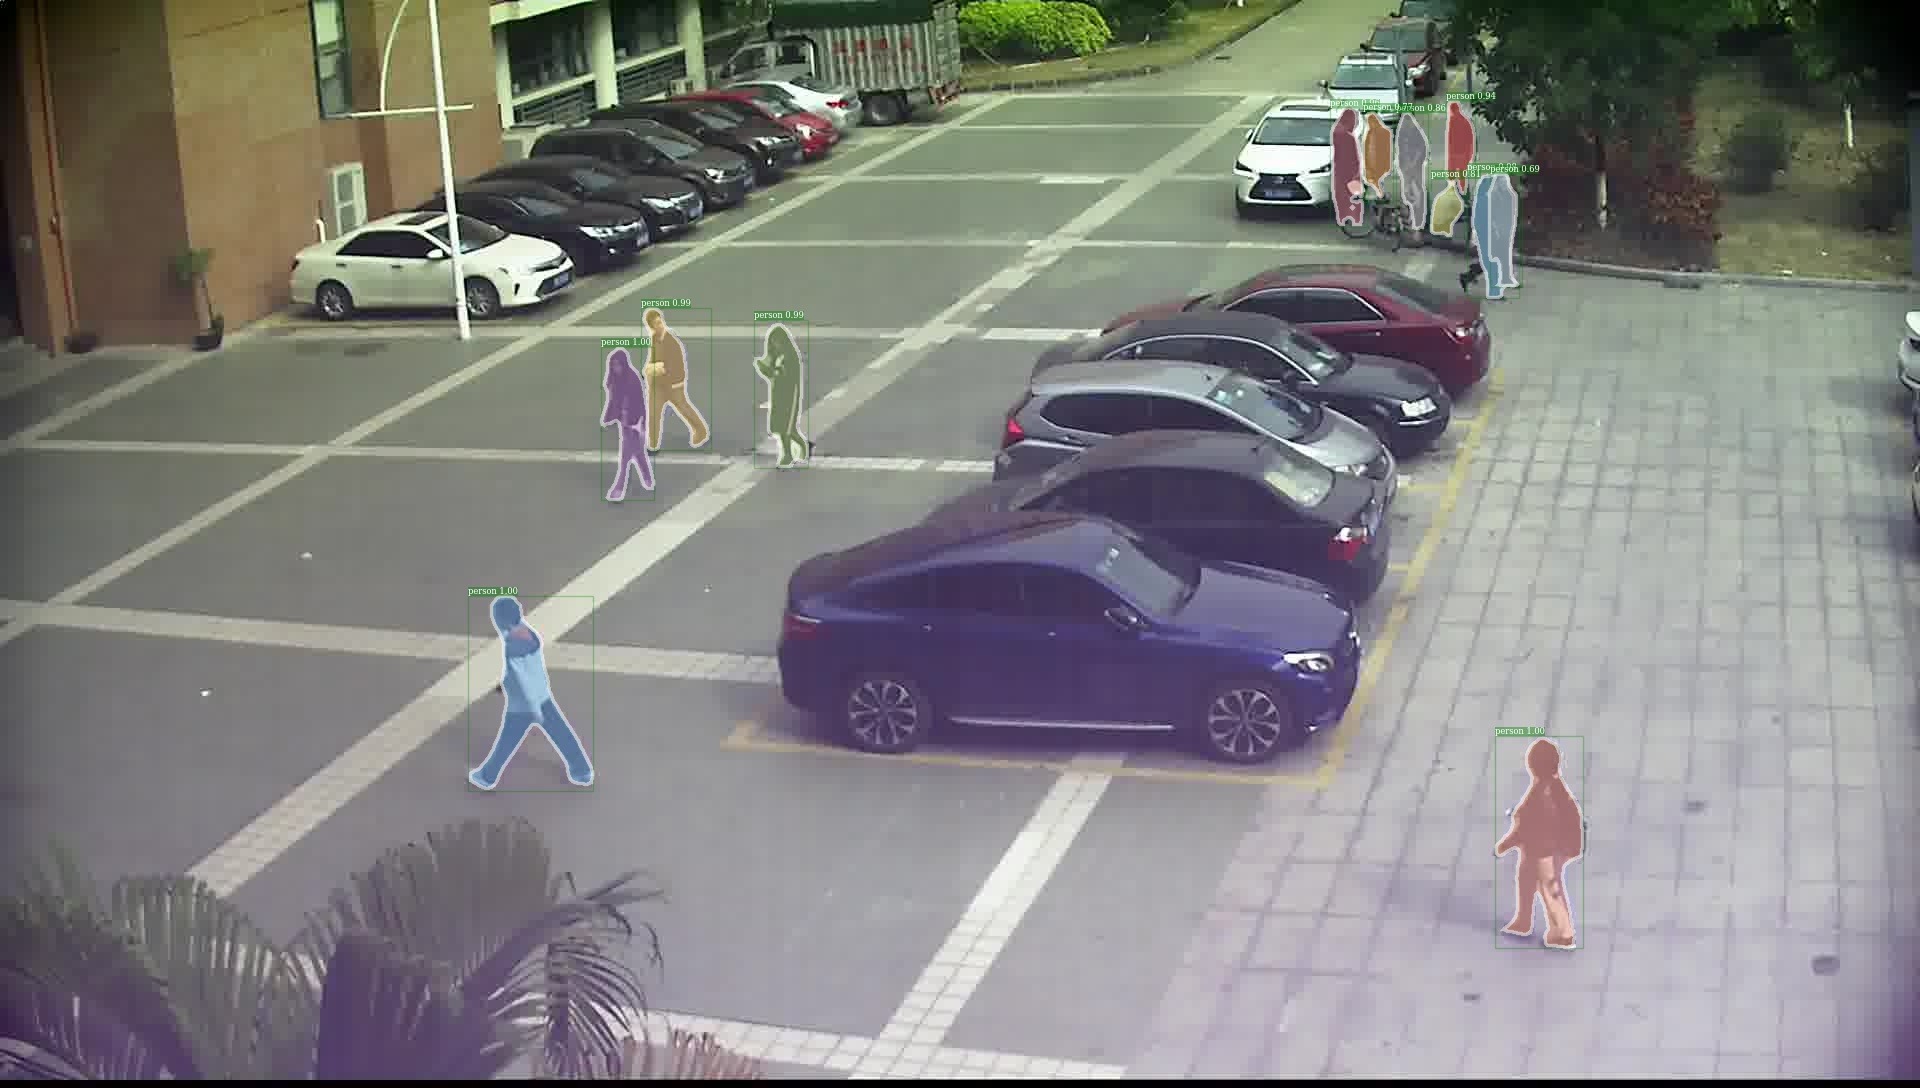
\includegraphics[width=0.3\linewidth]{figures/1-2_5_151_det.jpg}~
    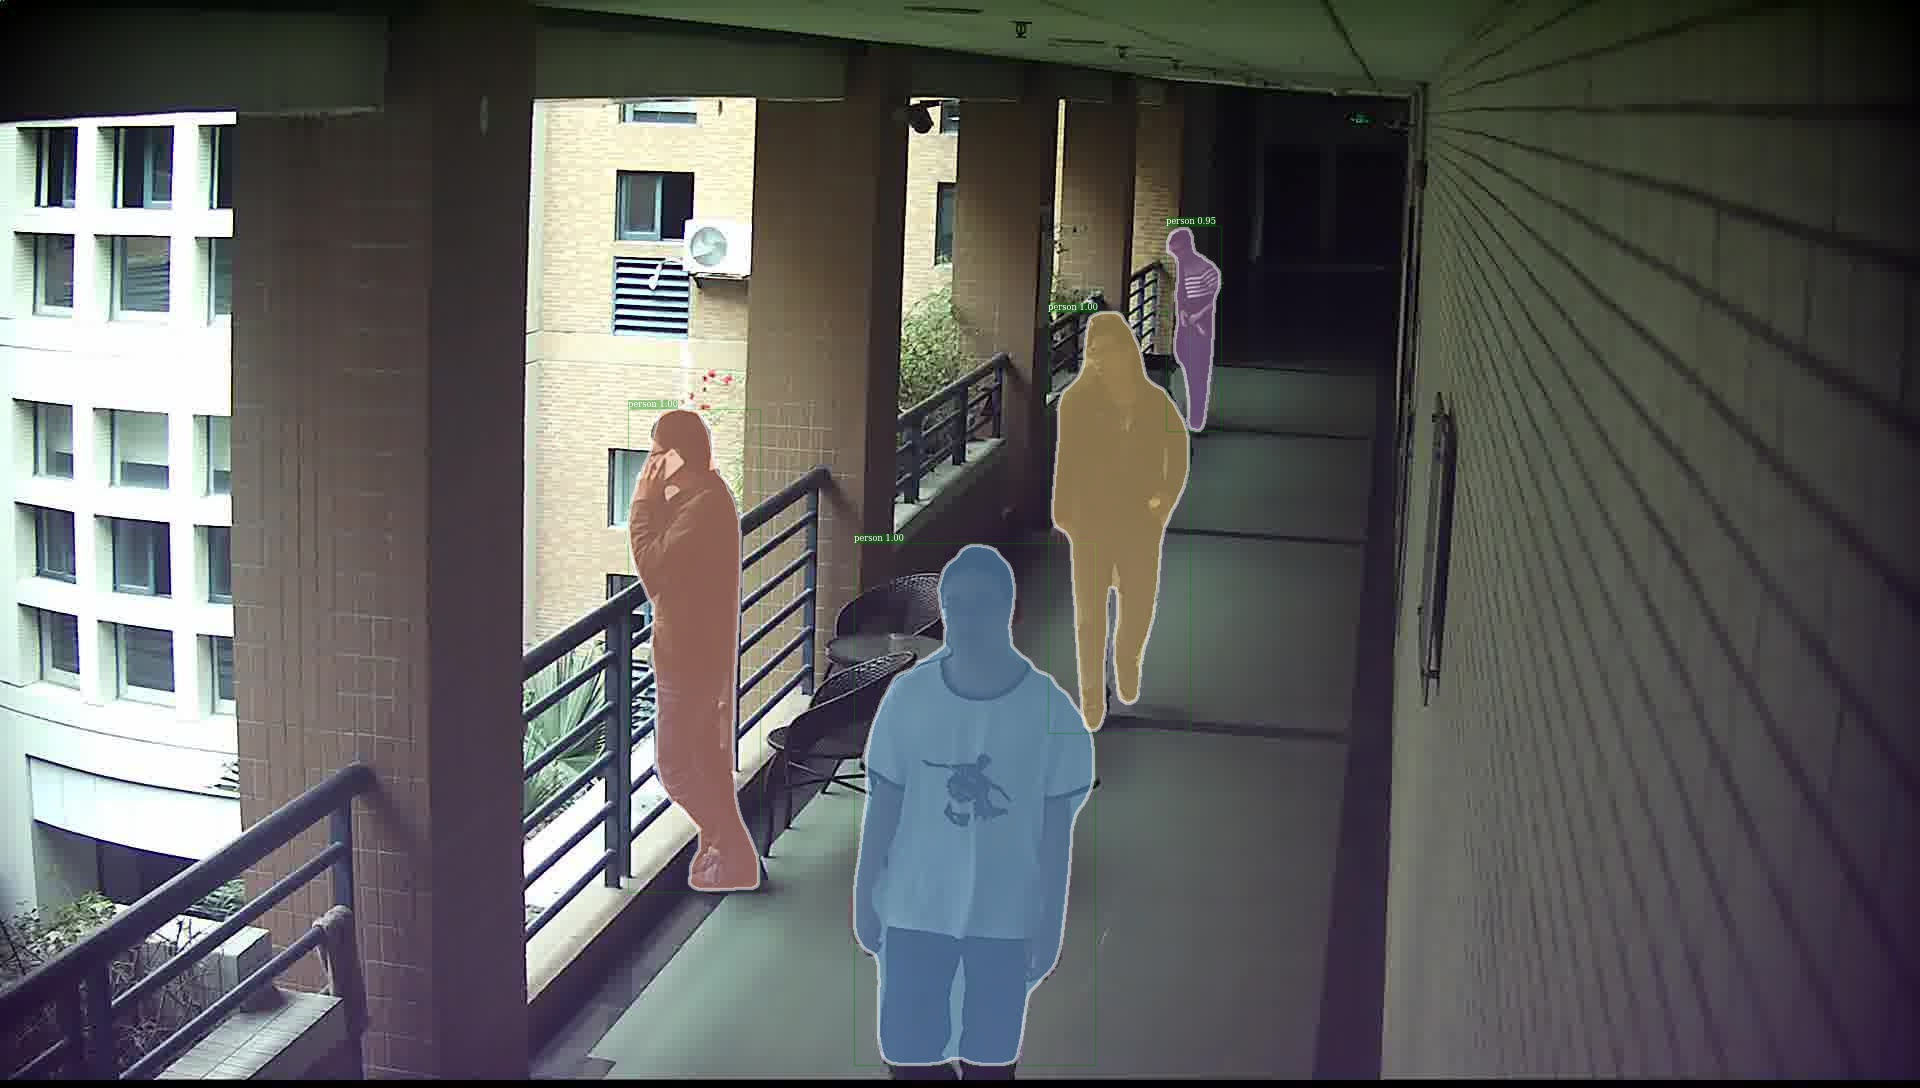
\includegraphics[width=0.3\linewidth]{figures/3-7_10_394_det.jpg}
    \caption{Detectron行人检测结果可视化}
    \label{fig:detectron}
    \end{figure}
    \end{frame}

\subsection{行人重识别论文复现}

    \begin{frame}{行人重识别论文复现结果}
    \begin{block}{}
    训练阶段交叉熵误差(Loss)随着数据集训练批次数(Epoch)变化曲线如图\ref{fig:loss}所示。
    行人重识别,指的是在多个视野不重叠的监控视频中,重新识别那些之前出现过的行人,即把当前行人与之前已标记的人物相对应。
    \end{block}
    \begin{columns}[]
    \centering
    \begin{column}{0.6\textwidth}
        \begin{table}
            \centering
            \begin{tabular}{@{}ccccc@{}}
            \toprule
                    & mAP   & Rank1 & Rank10 \\ \midrule
            论文中显示  & 77.3  & 92.4  & 97.9   \\
            复现结果   & 71.1  & 86.2  & 93.4   \\ \bottomrule
            \end{tabular}
            \caption{Market1501数据集测试结果}
            \label{tab:test}
        \end{table}
    \end{column}
    \begin{column}{0.3\textwidth}
        \begin{figure}[]
            \centering
            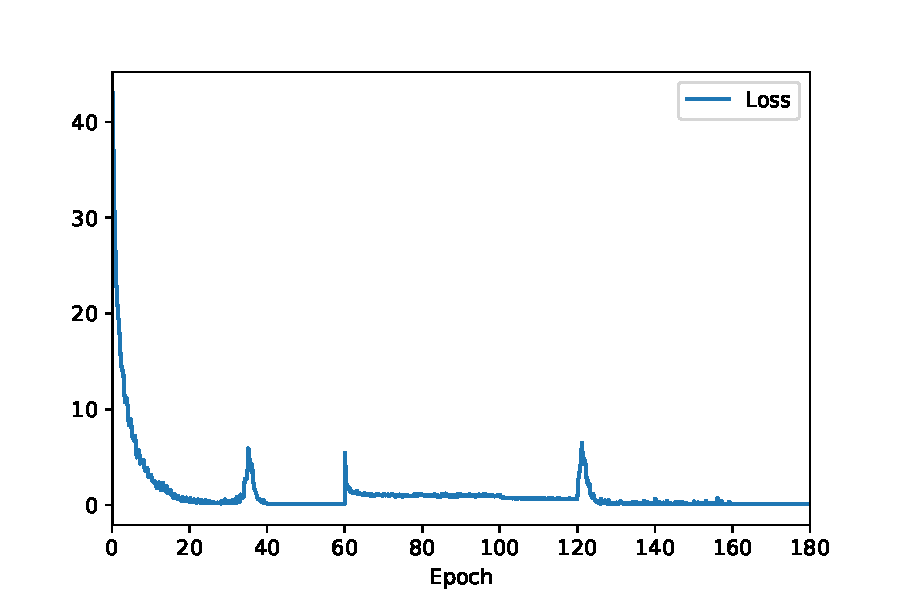
\includegraphics[width=\textwidth]{figures/loss}
            \caption{交叉熵误差随迭代数变化曲线}
            \label{fig:loss}
        \end{figure}
    \end{column}
    \end{columns}
    \end{frame}

    \begin{frame}{测试结果可视化}
        \begin{columns}
            \begin{column}{0.5\textwidth}
                图\ref{fig:testvis}是测试结果的可视化,左边一列是查询图片,每一张查询图片相应的右边一行是从测试库中挑选出来的图片,有红色边框的图片代表该人物标签与相应的查询图片人物标签不一致。
            \end{column}
            \begin{column}{0.5\textwidth}
                \begin{figure}
                \centering
                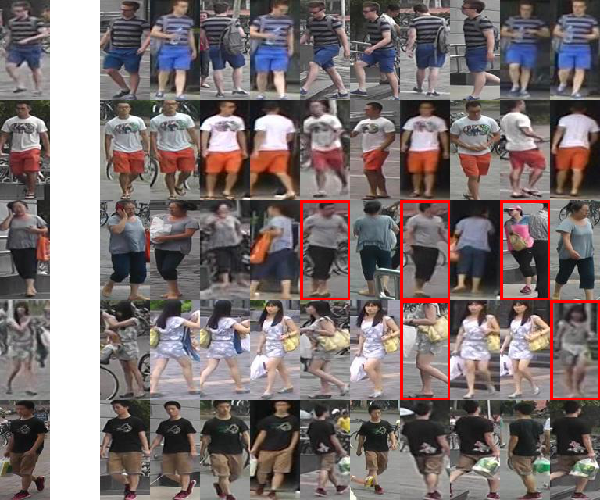
\includegraphics[width=\textwidth]{figures/vis3}
                \caption{测试结果可视化}
                \label{fig:testvis}
                \end{figure}
            \end{column}
        \end{columns}
    \end{frame}

\subsection{强化学习}

    \begin{frame}{经强化学习后选择的部署方案}
    \begin{block}{}
    使用Q-Learning算法,表\ref{tab:rlresult}为经过强化学习训练后的智能体在应对各种状态时,最有可能采取的行动统计。最优方案下的监控画面如图\ref{fig:rlresult}所示。
    \end{block}
    \begin{columns}
        \begin{column}{0.5\textwidth}
            \begin{table}
                \centering
                \begin{tabular}{@{}ccc@{}}
                \toprule
                方案               & 频次  & 占比      \\ \midrule
                (1, 2, 7, 10, 14) & 190 & 65.97\% \\
                (1, 2, 7, 10, 13) & 78  & 27.08\% \\
                (1, 2, 7, 9, 14)  & 18  & 6.15\%  \\
                (1, 3, 7, 10, 14) & 1   & 0.35\%  \\
                (0, 2, 7, 10, 14) & 1   & 0.35\%  \\ \bottomrule
                \end{tabular}
                \caption{学习后选择的部署方案}
                \label{tab:rlresult}
            \end{table}
        \end{column}
        \begin{column}{0.5\textwidth}
            \begin{figure}
            \centering
            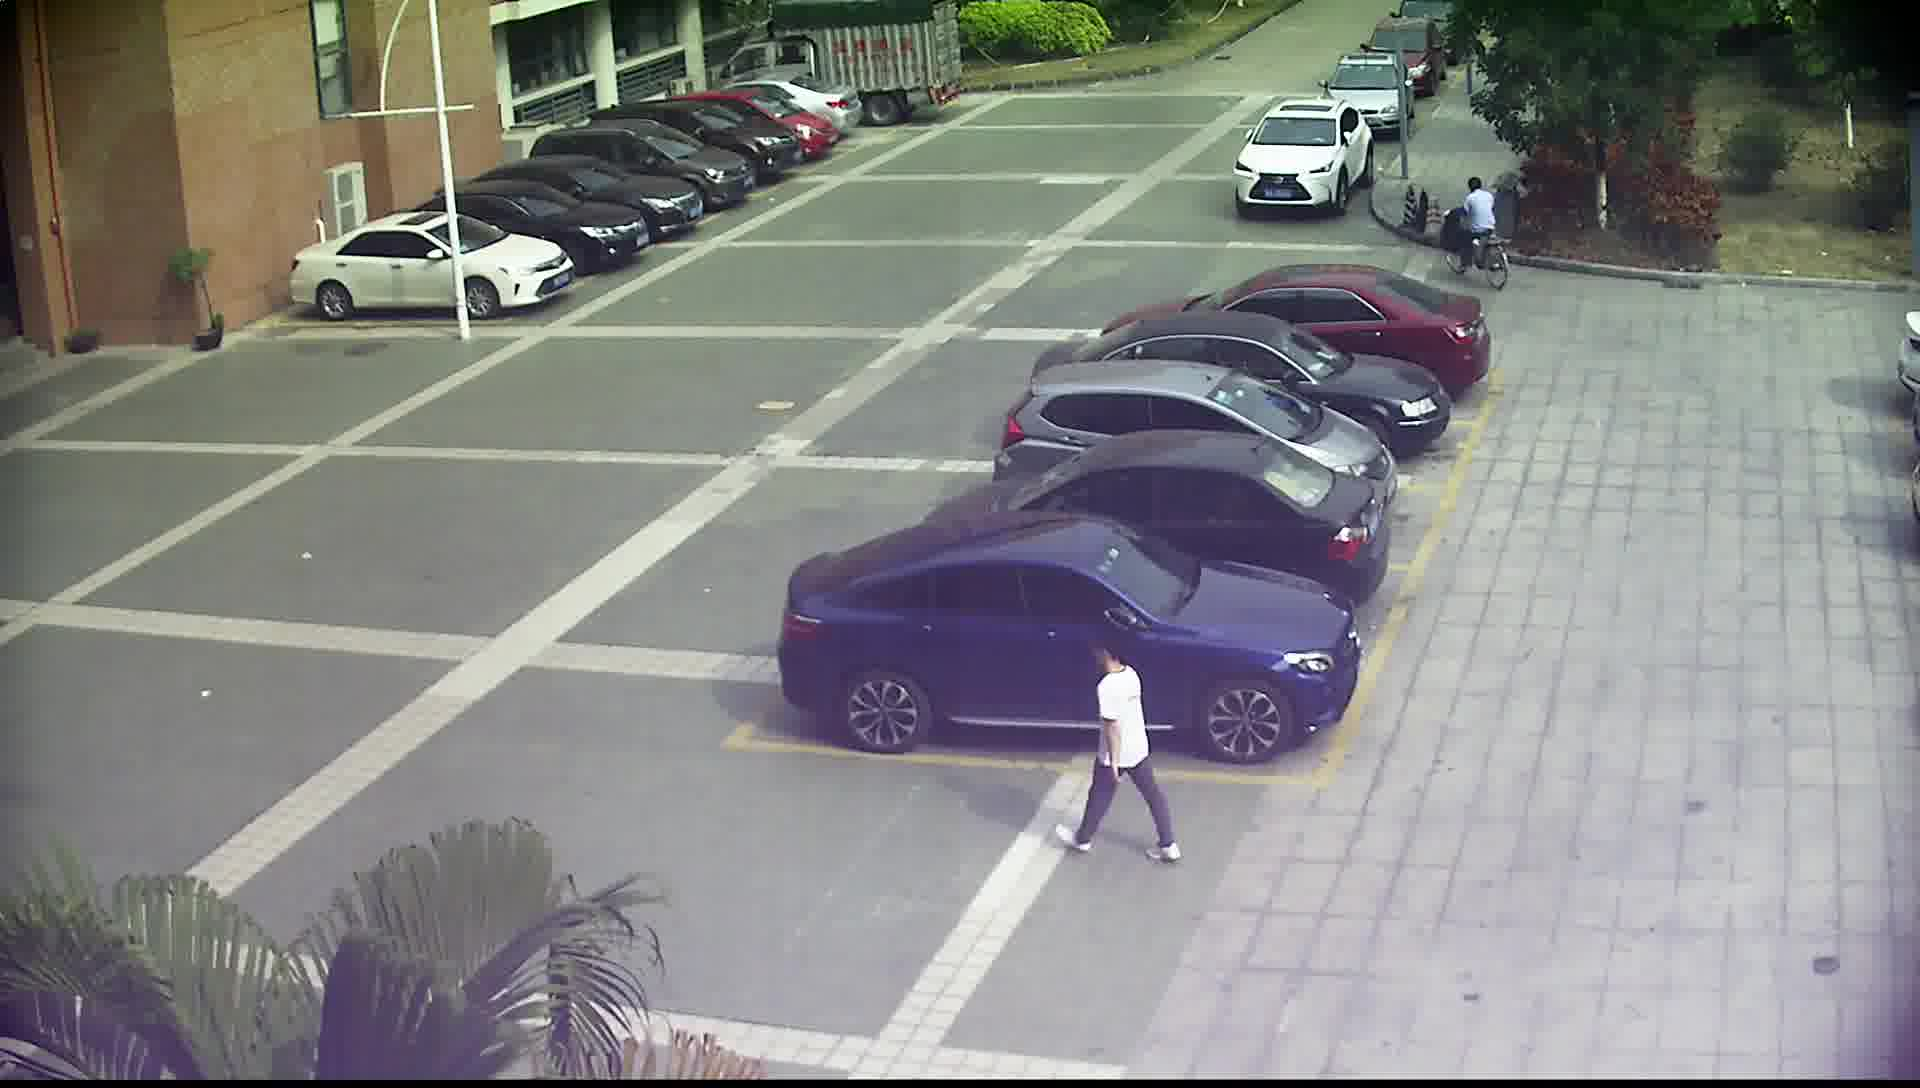
\includegraphics[width=0.3\textwidth]{figures/1-2}
            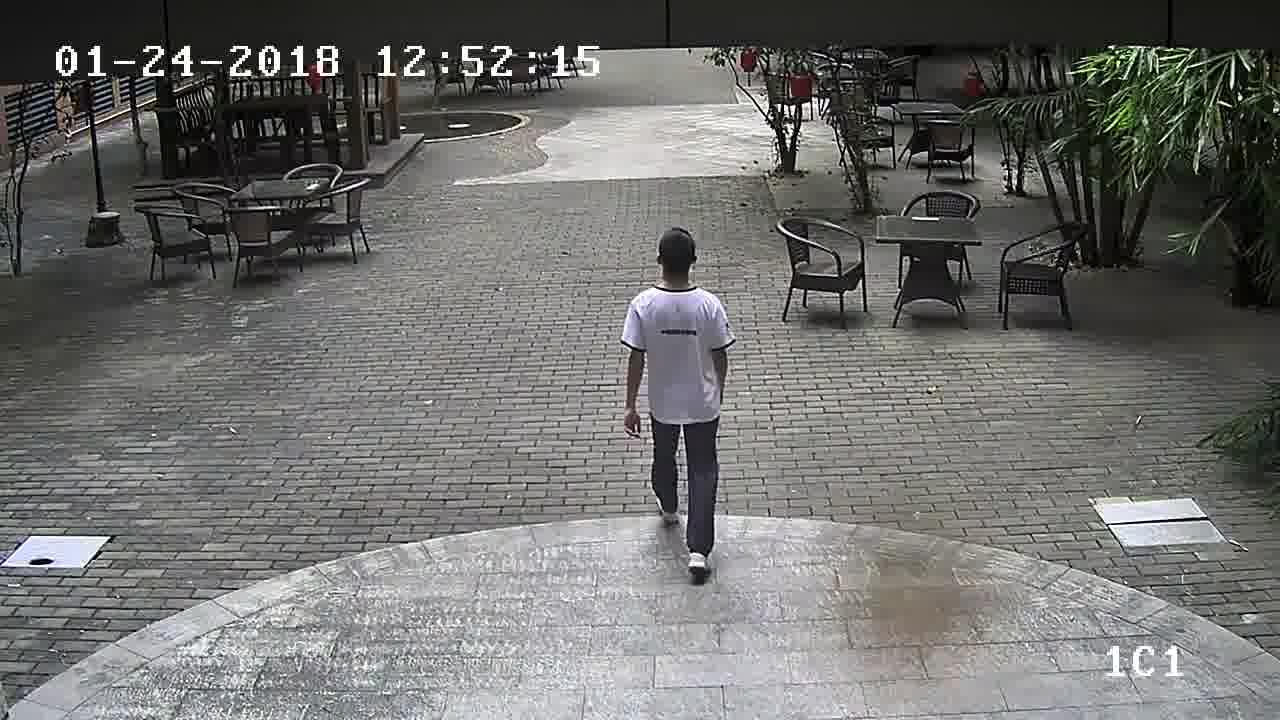
\includegraphics[width=0.3\textwidth]{figures/1-4}\\
            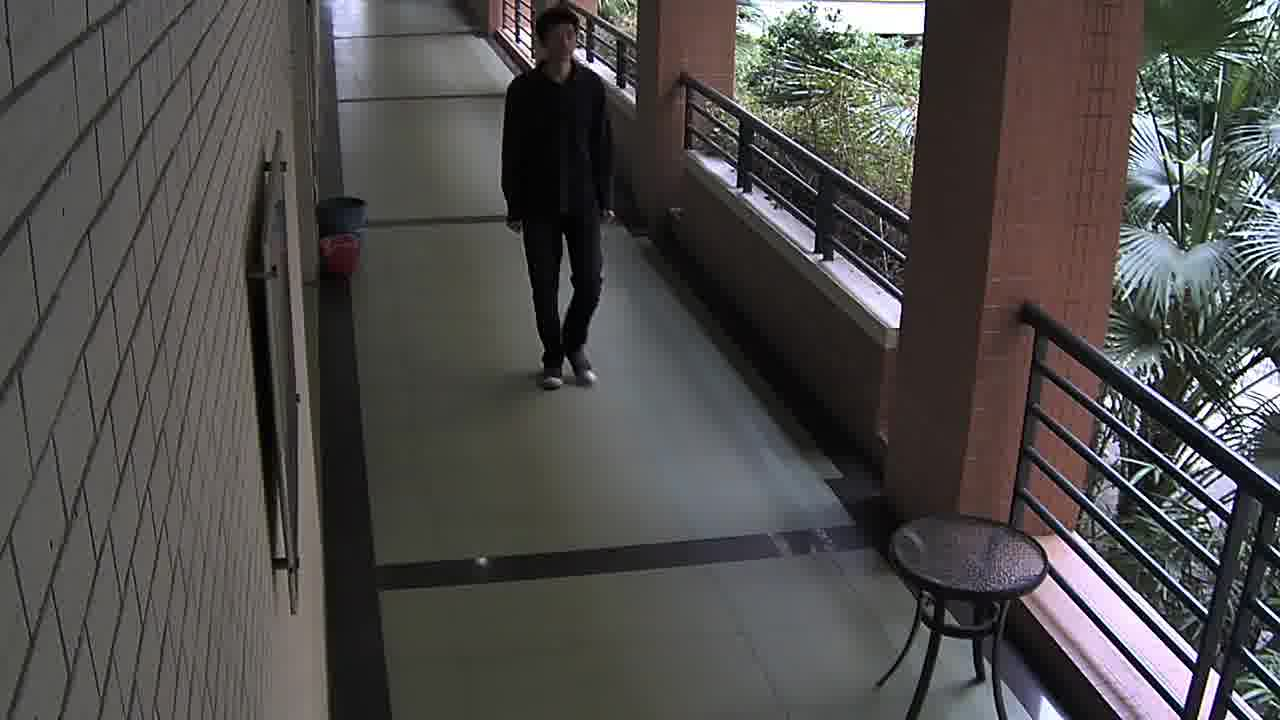
\includegraphics[width=0.3\textwidth]{figures/2-3}
            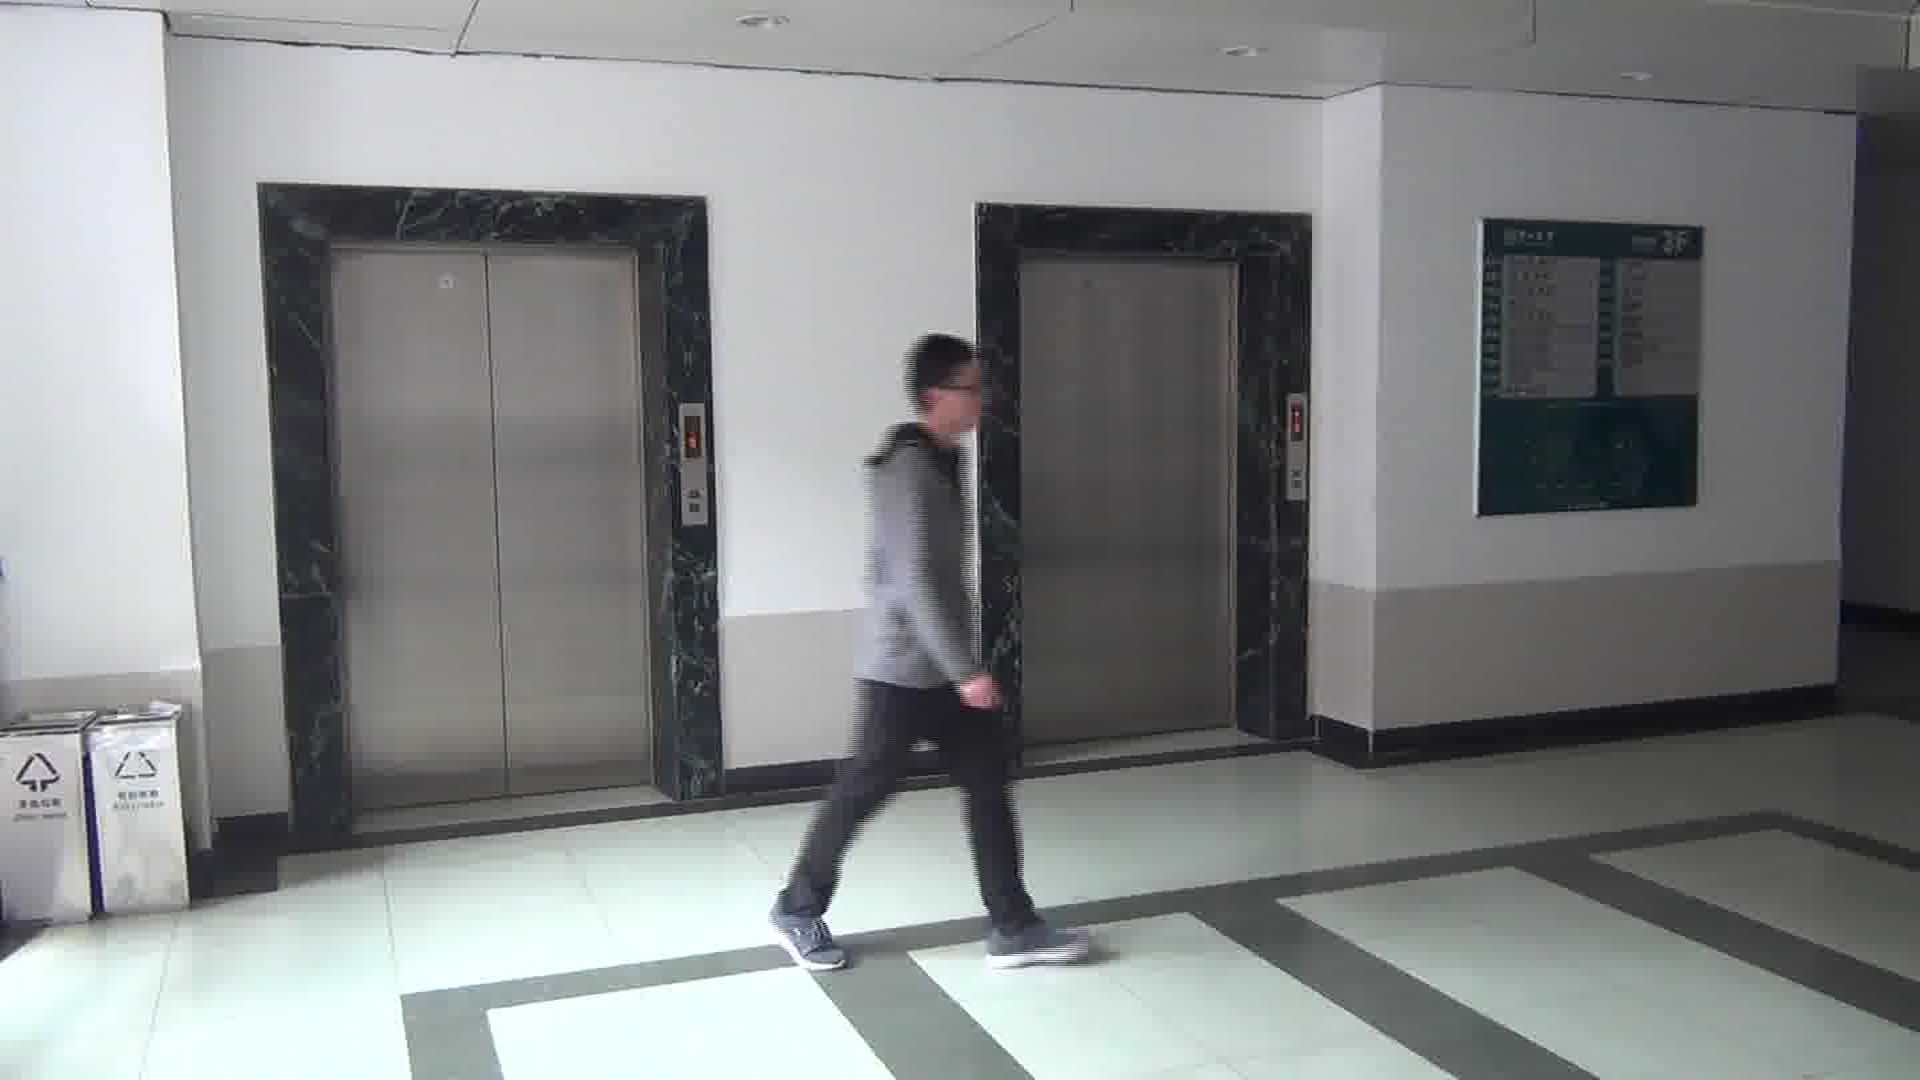
\includegraphics[width=0.3\textwidth]{figures/3-2}
            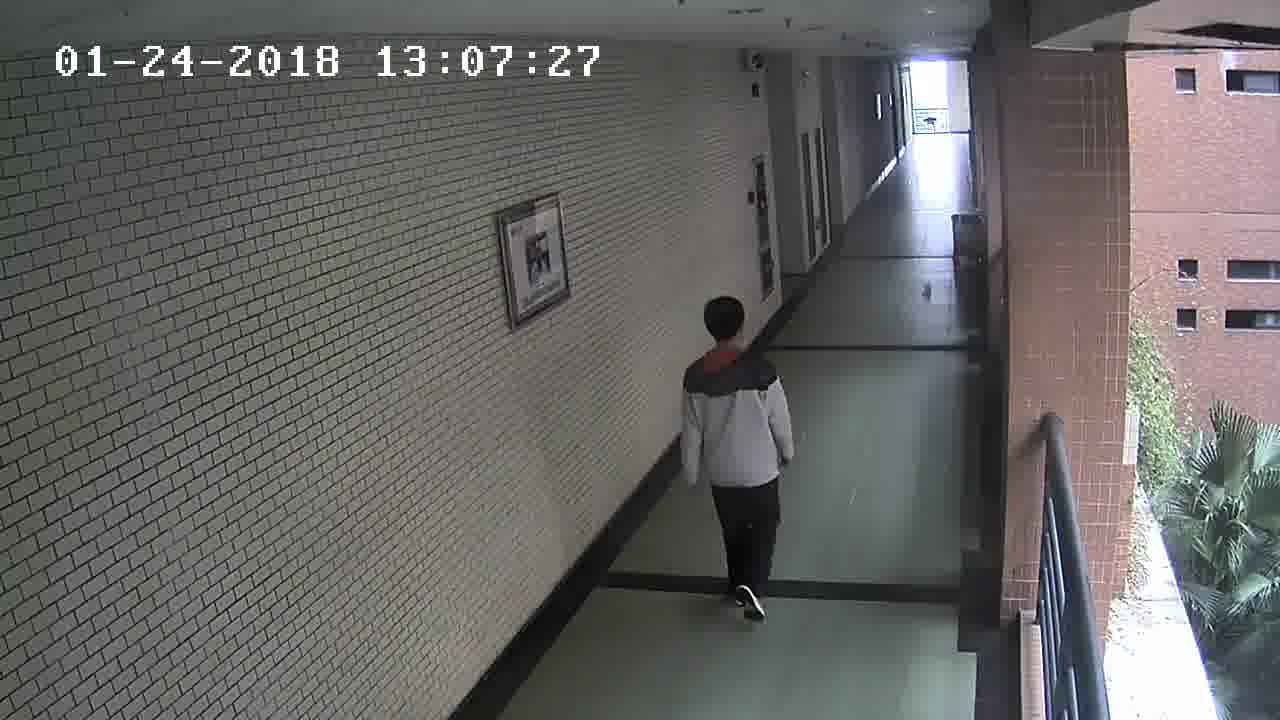
\includegraphics[width=0.3\textwidth]{figures/3-6}
            \caption{最优部署方案}
            \label{fig:rlresult}
            \end{figure}
        \end{column}
    \end{columns}
    \end{frame}


\section{理论框架}
项目的理论框架主要包括当前行人重识别领域state-of-the-art的算法思想、摄像头部署方案的评价指标以及强化学习模型在项目中的应用。

\subsection{行人重识别领域state-of-the-art的算法思想}

\subsubsection{Part-based Convolutional Baseline (PCB)}
这篇论文的Baseline采用了最近很热门的Part的思想,但不同于计算图片中的Attention,而是简单地将图片在垂直方向上分块,获取每一个块的特征。

图\ref{fig:baseline} 是Baseline的架构图。在Baseline中,模型以ResNet50作为Backbone Network。ResNet50模型首先在ImageNet数据集上训练至收敛,然后去掉为ImageNet分类任务而设计的全局池化层(Global Average Pooling Layer)及其后面的全连接层(Fully Connected Layer),使ResNet50模型成为一个高效的图像特征提取器,其中的特征既包括颜色、纹理、形状等视觉特征,也包括类别、姿势、性别等语义特征。作为一个端到端(End-to-End)的特征提取器,其输入为包含RGB通道的原始图像,输出为包含2048个通道(2048 Channels)的Feature Maps。

将ResNet50模型输出的Feature Maps在竖直方向上分成$p=6$个水平条(Horizontal Stripes),每个通道(Channel)保持独立。每个水平条通过一个尺寸与水平条尺寸相同全局池化层,使得原本为矩形的水平条变为一个$1\times1$的像素点,再将其与同一水平条其他通道的像素点拼接起来得到一个$2048\times1\times1$的向量。因为每个水平条会得到一个特征向量,所以经过全局池化层之后可得到$p$个向量,每一个向量都能表示原图像在对应的水平条范围内的局部特征。此方法的优点是简单、高效、易实现,缺点是每个人各部位的分布不同,人物上所具备的关注点也千差万别,将Feature Maps在竖直方向上均匀分割不能很好地体现人与人之间的这些差异。

得到$p$个2048维的特征向量之后,再使用核尺寸为$1\times1$的卷积层将每个2048维的向量降为256维,以减少之后分类任务的计算量。每一个局部特征向量后接一个$n$分类器以预测该图像的类别,其中$n$为训练集中label的个数。训练的损失函数(Loss Function)使用交叉熵损失(Cross Entropy Loss)。

在测试阶段,也即特征提取阶段,将最后的$p$个$n$分类器去掉,直接将$p$个256维的向量拼接(concatenate)为向量$\textbf g$或将$p$个2048维的向量拼接为向量$\textbf h$作为原始行人图像的特征表示。

\subsubsection{Refined Part Pooling (RPP)}
Part-based Convolutional Baseline (PCB) 将Feature Maps在竖直方向上均匀分成$p$个水平条,以获得行人各部位的特征。此方法有操作简单、运算量少、易于实现的优点,但忽略了人与人之间各部位的位置差距。因此,有必要在Baseline的基础上进行改进,不再局限于一个规范的矩形,而是通过计算判断每一个像素点「应该属于」哪一个部分。对于不同通道、相同位置的像素点,进行统一处理。

于是目标就成了:给定一个列向量(column vector,表示不同通道、相同位置的像素点),判断其属于哪一个部分。这就变成了一个分类问题。在这里使用一个线性神经网络层,来将所有的列向量分类。线性神经网络层有权重$W$和偏置$b$组成,为了简化表示,这里省略偏置$b$。对于一个列向量$f$,其属于第$i$个部分的概率$P(p_i|f)$为:
\begin{equation}
P(p_i|f)=\mathop{\rm softmax}\left(W_i^{\rm T}f\right)=\frac{\exp\left(W_i^{\rm T}f\right)}{\sum_j^p\exp\left(W_j^{\rm T}f\right)}
\end{equation}
其中$p_i$表示Feature Map的第$i$部分。

在PCB中,列向量$f$只绝对的属于某一个部分。在求得$P(p_i|f)$后,则可将原始的列向量$f$按照概率分布分配到各部分。对于第$i$个部分$p_i$,其计算方式为:
\begin{equation}
p_i=\frac{1}{H\times W}\sum_{j=1}^{H\times W}P(p_i|f_j)\times f_j
\end{equation}
其中$H$、$W$分别代表Feature Map的高和宽。

如图\ref{fig:refined}所示。

完整的PCB+RPP架构图如图\ref{fig:structure2}所示。

\subsection{摄像头部署方案的评价指标}

\subsection{强化学习模型}

\subsection{面向CPU集群的分布式深度学习训练框架}

\begin{figure}
\centering
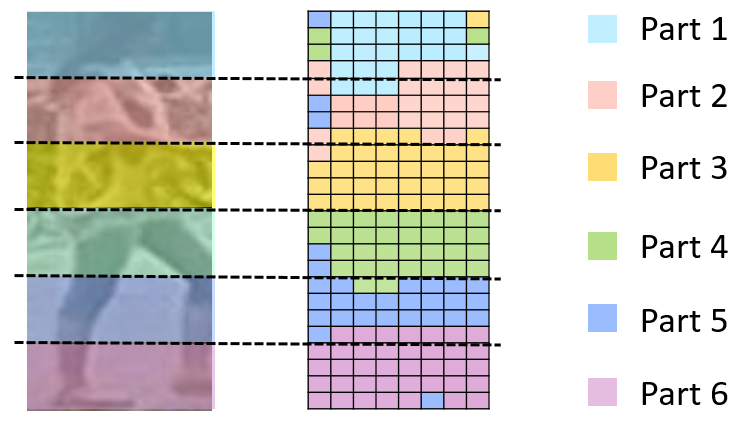
\includegraphics[width=0.6\textwidth]{figure/outliers1}
\caption{Refined Part Pooling示意图}
\label{fig:refined}
\end{figure}

\begin{figure}
\centering
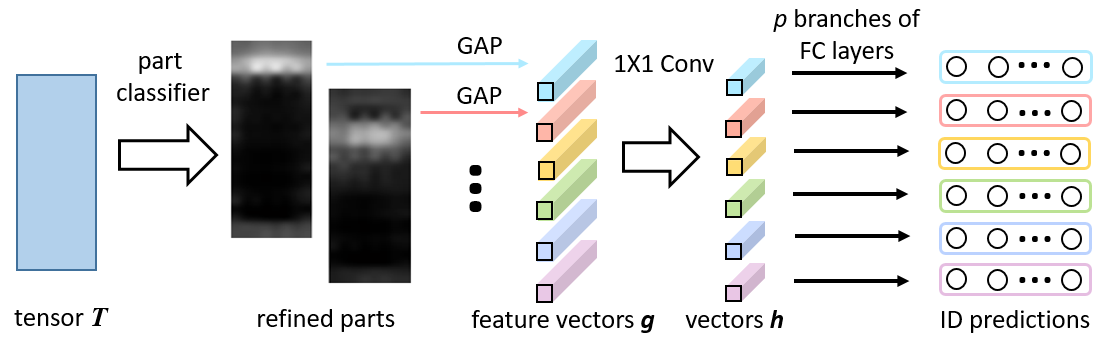
\includegraphics[width=1\textwidth]{figure/structure2}
\caption{PCB+RPP架构图}
\label{fig:structure2}
\end{figure}

%\xdbg%末页致谢
\frame[plain, noframenumbering]{\finalpage{{\huge 谢谢!}}}

\end{document}
